\documentclass[twocolumn]{revtex4}
\usepackage[]{graphicx}
\begin{document}
\title{
Velociraptors and Humans Chase: Updated
}

\author{J.~Van Slycke}
\affiliation{Siena College, Loudonville, NY}
\date{\today}

\begin{abstract}
  
    In this project, students were given the assignment to track the outcomes of a scenario where a human is being traced by a velociraptor. Raptology explains that 'raptors will start to attack when one meter away from their prey and try only three times to bite before giving up. In this 4 part project, we had to find and plot when the velociraptor and human would cross paths, find when the velociraptor would be within attacking distance, and finally what the probability was that a human would survive the attack. Our results showed that the raptor would be one meter behind the human after 1.94 seconds when the human was at 35.82 meters and caught up to the human after 2 seconds at 36 meters. There was approximately a 62 percent chance of survival, but tested results varied between 59 and 65 percent. 
\end{abstract}

\maketitle
     
	\section{Part I}

	The point of section I was to plot the respective graphs of distance traveled over time for both the velociraptor and the human. To do this, I created an empty list [x], and used the append function to add numbers to the list. The range went up to 500, and then before appending to the list, I divided each number by 100 so that the list would step up in increments of .01. I then created lists for both the human [y] and the raptor [z], tracking their distance with respects to the time passing [x]. The equation for the human looked like $$y1=3*i +30$$ and the equation for the velociraptor was $$z1=18*i$$with 'i' being all the values in the list [x]. I then appended y1 to the empty list [y], and z1 to [z], giving all the distance values.
	
	\begin{figure}[h]
		\centering 
		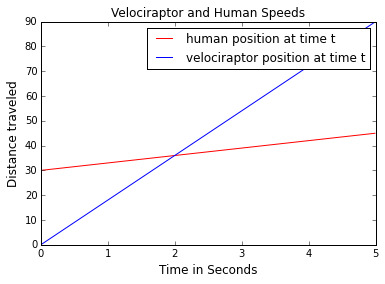
\includegraphics[width=.4\textwidth]{1_plot}
	\end{figure}
	This plot gave an accurate estimation and visual representation of the distance the raptor and human can travel with accordance to time. By using lists for the points, it set me up for problems two and three.
	\section{Part II}
	In part II, I had to use python code to give an exact answer for when the velociraptor caught up to the human. To do this, I created a for loop that compared the values of the velociraptor and human together and had the loop print x[i] (the time) and y[i] (the human's distance) when the two lists had a number that was equal. This looked like $$ y[i]==z[i]$$ The range in my loop had to go up to 500 because the loops that tracked the distance the human and velociraptor traveled went up in increments of .01 due to the list [x]. 

\section{Part III}
Part III was where things started to get interesting. In this section, we had to use our code to find out where the human was when the velociraptor was one meter behind, and how much time had passed at that point. To do this, I created yet another for loop that compared the values of the velociraptor and human together and had the loop print x[i] (the time) and y[i] (the human's distance) when the difference between the human's distance minus that of the velociraptor's was less than 1 meter. This looked like $$y[i]-z[i]<=1$$ The range in this loop also went up to 500, for the same reason as mentioned in part II. I then plotted a graph with an arrow showing the point on the graph when the velociraptor was 1 meter behind. 
	\begin{figure}[h]
		\centering 
		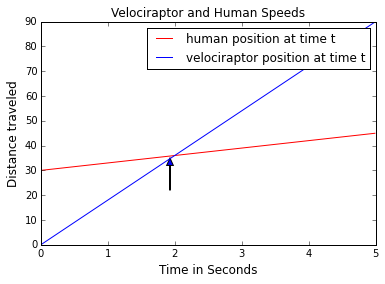
\includegraphics[width=.4\textwidth]{2_plot}
	\end{figure}
	This plot gave an accurate, if not exact estimation and visual representation of the distance the human had traveled when the velociraptor was one meter behind. 
	
\section{Part IV}
Part IV was the most important of all parts because it tested the probability of life if a human were to be chased by a velociraptor. To do this, I created a function, escaping. Escaping created 3 random integers up to 100, each integer representing a different bite. If the first integer returned a number less than or equal to 20, or the second integer returned a number less than or equal to 15, or the third integer returned a number less than or equal to 7, it would return the string "Velociraptor gets you!" If none of those booleans were true, the function would return "You Live!" I then made a for loop that goes from 0 to 1000, each time running the escaping function. Everytime the result from 'escaping' equaled "Velociraptor gets you!" failures added one. Otherwise, successes added one. In the end, I divided successes by 1000, and printed the probability of life.

\section{Conclusion}
This project gave solid results that prove it is indeed possible, likely even, to escape a velociraptor attack. Not beause you will be faster than them, because you won't be; but because velociraptors happen to be terrible at getting a grip on their two-legged prey (and they get frustrated easily). So if you ever find yourself on the island in Jurassic Park, keep your eyes open, and pray that you are one of the ~60 percent of people that escape.
	

\end{document}